\documentclass{standalone}
\usepackage{tikz}
\usetikzlibrary{patterns, positioning}
\usepackage[sfdefault]{ClearSans} %% option 'sfdefault' activates Clear Sans as the default text font
\usepackage[T1]{fontenc}

\begin{document}
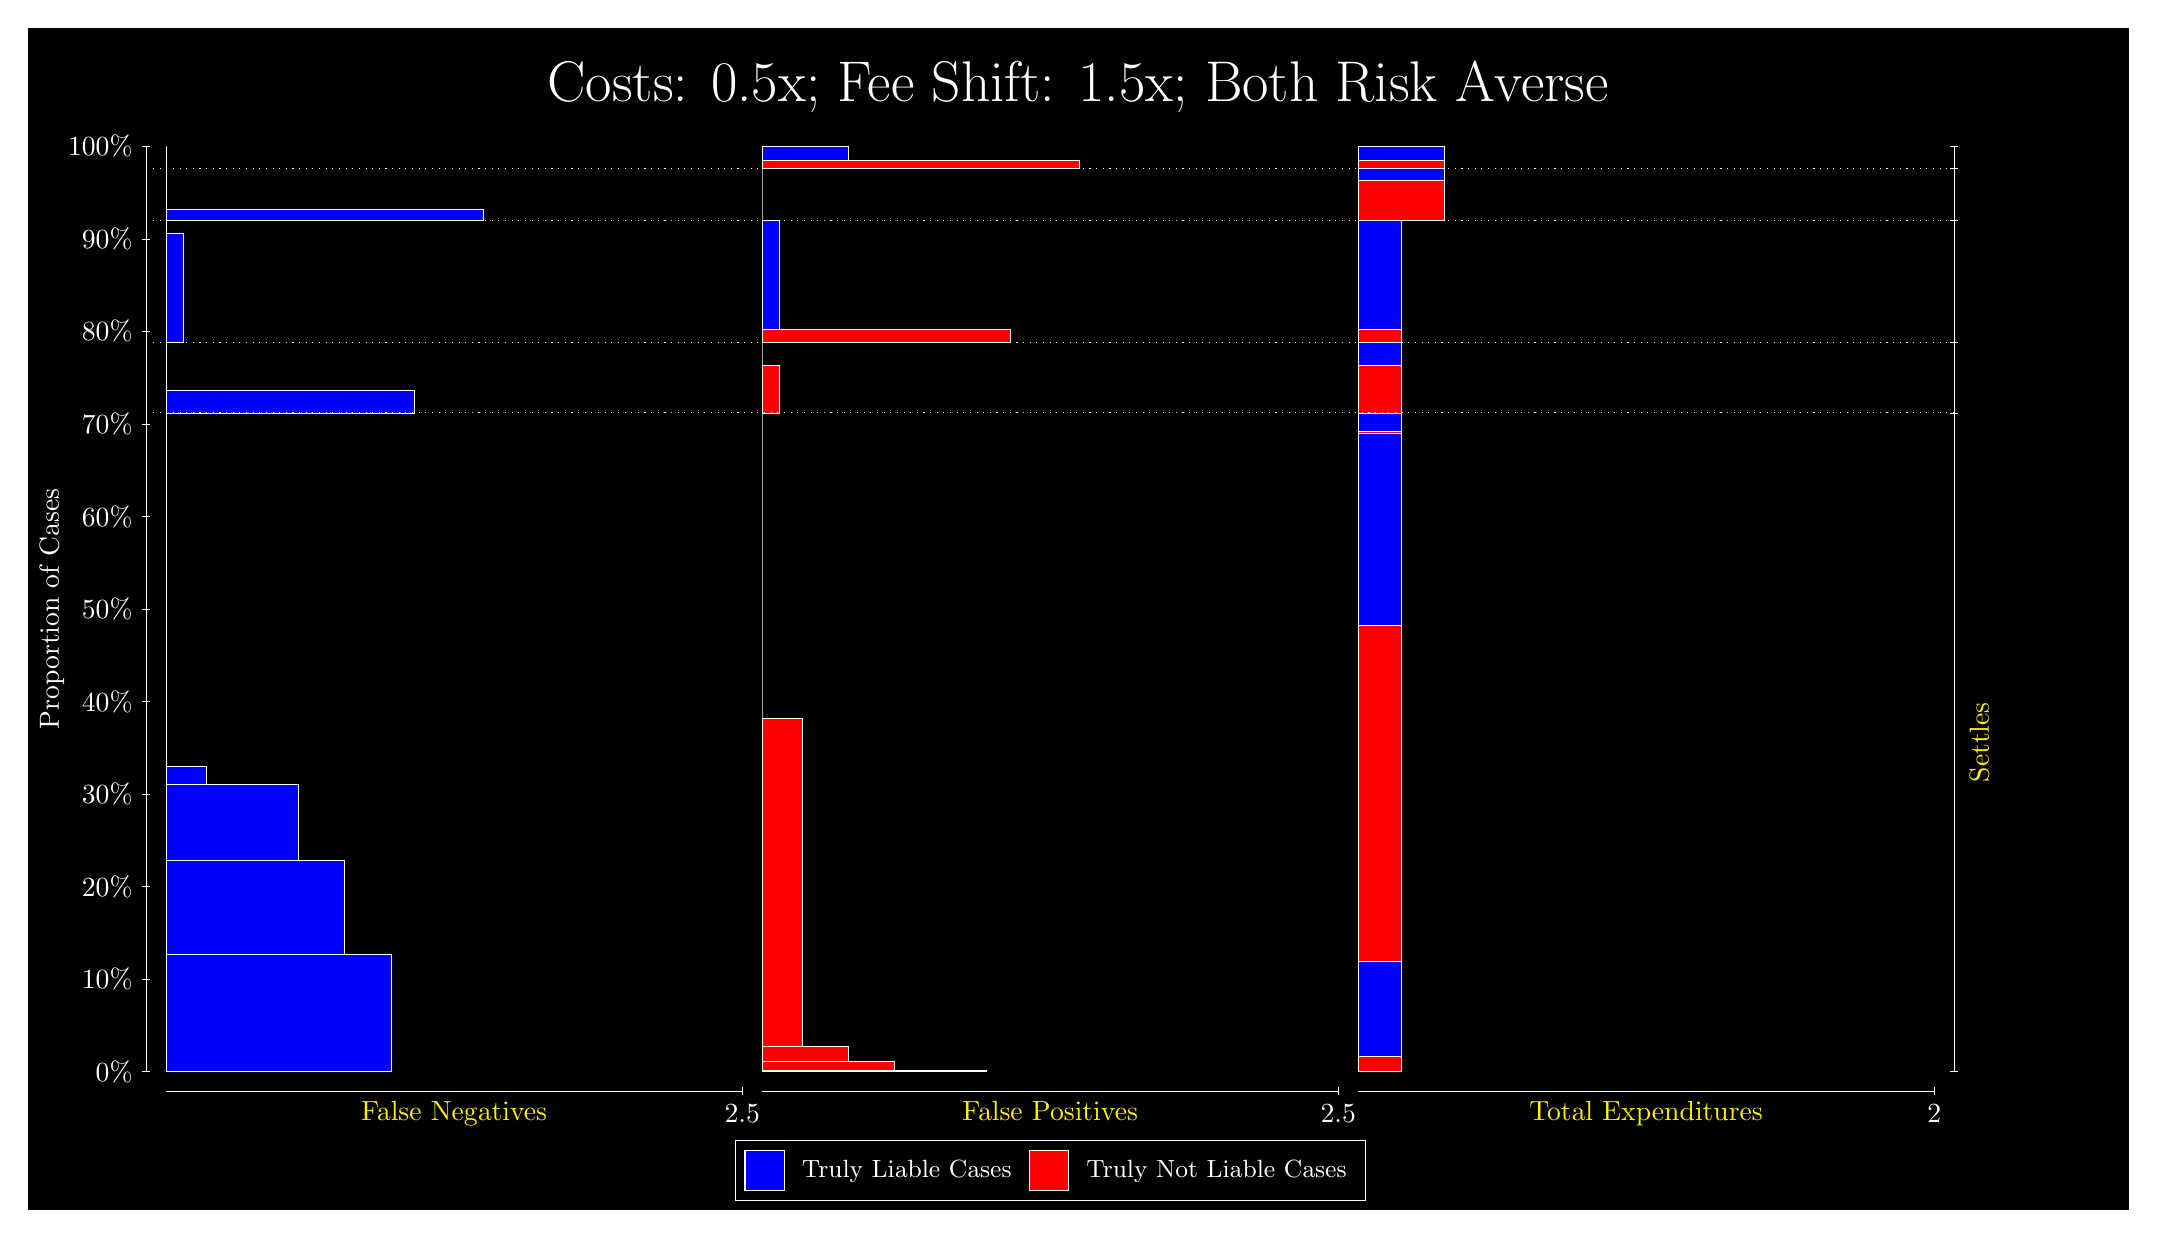
\begin{tikzpicture}
\draw[fill=black] (0,0) rectangle (26.667,15);
\draw[text=white] (0,13.5) rectangle (26.667,15) node[midway] {\huge Costs: 0.5x; Fee Shift: 1.5x; Both Risk Averse};
\draw[white, very thin] (1.5,1.75) -- (1.5,13.5);
\node[rotate=90, text=white, anchor=center] at (0.3, 7.625) {Proportion of Cases};
\draw[white, very thin] (1.45,1.75) -- (1.55,1.75);
\node[text=white, anchor=east] at (1.45, 1.75) {0\%};
\draw[white, very thin] (1.45,2.925) -- (1.55,2.925);
\node[text=white, anchor=east] at (1.45, 2.925) {10\%};
\draw[white, very thin] (1.45,4.1) -- (1.55,4.1);
\node[text=white, anchor=east] at (1.45, 4.1) {20\%};
\draw[white, very thin] (1.45,5.275) -- (1.55,5.275);
\node[text=white, anchor=east] at (1.45, 5.275) {30\%};
\draw[white, very thin] (1.45,6.45) -- (1.55,6.45);
\node[text=white, anchor=east] at (1.45, 6.45) {40\%};
\draw[white, very thin] (1.45,7.625) -- (1.55,7.625);
\node[text=white, anchor=east] at (1.45, 7.625) {50\%};
\draw[white, very thin] (1.45,8.8) -- (1.55,8.8);
\node[text=white, anchor=east] at (1.45, 8.8) {60\%};
\draw[white, very thin] (1.45,9.975) -- (1.55,9.975);
\node[text=white, anchor=east] at (1.45, 9.975) {70\%};
\draw[white, very thin] (1.45,11.15) -- (1.55,11.15);
\node[text=white, anchor=east] at (1.45, 11.15) {80\%};
\draw[white, very thin] (1.45,12.325) -- (1.55,12.325);
\node[text=white, anchor=east] at (1.45, 12.325) {90\%};
\draw[white, very thin] (1.45,13.5) -- (1.55,13.5);
\node[text=white, anchor=east] at (1.45, 13.5) {100\%};

\draw[white, very thin] (24.457,1.75) -- (24.457,13.5);
\draw[white, very thin] (24.407,1.75) -- (24.507,1.75);
\node[anchor=west] at (24.407, 1.75) {};
\draw[white, very thin] (24.407,10.114) -- (24.507,10.114);
\node[anchor=west] at (24.407, 10.114) {};
\draw[white, very thin] (24.407,11.012) -- (24.507,11.012);
\node[anchor=west] at (24.407, 11.012) {};
\draw[white, very thin] (24.407,12.559) -- (24.507,12.559);
\node[anchor=west] at (24.407, 12.559) {};
\draw[white, very thin] (24.407,13.215) -- (24.507,13.215);
\node[anchor=west] at (24.407, 13.215) {};
\draw[white, very thin] (24.407,13.5) -- (24.507,13.5);
\node[anchor=west] at (24.407, 13.5) {};

\draw[white, very thin, fill=blue] (1.75,1.75) rectangle (4.6044,3.2379);
\draw[white, very thin, fill=blue] (1.75,3.2379) rectangle (4.0188,4.4365);
\draw[white, very thin, fill=blue] (1.75,4.4365) rectangle (3.4333,5.392);
\draw[white, very thin, fill=blue] (1.75,5.392) rectangle (2.2623,5.6298);
\draw[white, very thin, fill=red] (1.75,5.6298) rectangle (1.75,10.114);
\draw[white, very thin, fill=blue] (1.75,10.114) rectangle (4.8971,10.408);
\draw[white, very thin, fill=red] (1.75,10.408) rectangle (1.75,11.012);
\draw[white, very thin, fill=blue] (1.75,11.012) rectangle (1.9696,12.392);
\draw[white, very thin, fill=red] (1.75,12.392) rectangle (1.75,12.559);
\draw[white, very thin, fill=blue] (1.75,12.559) rectangle (5.7754,12.703);
\draw[white, very thin, fill=red] (1.75,12.703) rectangle (1.75,13.215);
\draw[white, very thin, fill=red] (1.75,13.215) rectangle (1.75,13.324);
\draw[white, very thin, fill=blue] (1.75,13.324) rectangle (1.75,13.5);
\draw[white, very thin, fill=red] (9.3189,1.75) rectangle (12.173,1.7639);
\draw[white, very thin, fill=red] (9.3189,1.7639) rectangle (11.002,1.8755);
\draw[white, very thin, fill=red] (9.3189,1.8755) rectangle (10.417,2.0722);
\draw[white, very thin, fill=red] (9.3189,2.0722) rectangle (9.8312,6.2338);
\draw[white, very thin, fill=blue] (9.3189,6.2338) rectangle (9.3189,10.114);
\draw[white, very thin, fill=red] (9.3189,10.114) rectangle (9.5384,10.717);
\draw[white, very thin, fill=blue] (9.3189,10.717) rectangle (9.3189,11.012);
\draw[white, very thin, fill=red] (9.3189,11.012) rectangle (12.466,11.178);
\draw[white, very thin, fill=blue] (9.3189,11.178) rectangle (9.5384,12.559);
\draw[white, very thin, fill=red] (9.3189,12.559) rectangle (9.3189,13.071);
\draw[white, very thin, fill=blue] (9.3189,13.071) rectangle (9.3189,13.215);
\draw[white, very thin, fill=red] (9.3189,13.215) rectangle (13.344,13.324);
\draw[white, very thin, fill=blue] (9.3189,13.324) rectangle (10.417,13.5);
\draw[white, very thin, fill=red] (16.888,1.75) rectangle (17.437,1.9467);
\draw[white, very thin, fill=blue] (16.888,1.9467) rectangle (17.437,3.1453);
\draw[white, very thin, fill=red] (16.888,3.1453) rectangle (17.437,7.4185);
\draw[white, very thin, fill=blue] (16.888,7.4185) rectangle (17.437,9.8619);
\draw[white, very thin, fill=red] (16.888,9.8619) rectangle (17.437,9.8758);
\draw[white, very thin, fill=blue] (16.888,9.8758) rectangle (17.437,10.114);
\draw[white, very thin, fill=red] (16.888,10.114) rectangle (17.437,10.717);
\draw[white, very thin, fill=blue] (16.888,10.717) rectangle (17.437,11.012);
\draw[white, very thin, fill=red] (16.888,11.012) rectangle (17.437,11.178);
\draw[white, very thin, fill=blue] (16.888,11.178) rectangle (17.437,12.559);
\draw[white, very thin, fill=red] (16.888,12.559) rectangle (17.986,13.071);
\draw[white, very thin, fill=blue] (16.888,13.071) rectangle (17.986,13.215);
\draw[white, very thin, fill=red] (16.888,13.215) rectangle (17.986,13.324);
\draw[white, very thin, fill=blue] (16.888,13.324) rectangle (17.986,13.5);
\draw[white, dotted] (1.5,10.114) -- (24.457,10.114);
\draw[white, dotted] (1.5,11.012) -- (24.457,11.012);
\draw[white, dotted] (1.5,12.559) -- (24.457,12.559);
\draw[white, dotted] (1.5,13.215) -- (24.457,13.215);
\draw[white, very thin] (1.75,1.5) -- (9.0689,1.5);
\node[text=yellow, anchor=north] at (5.4094, 1.5) {False Negatives};
\draw[white, very thin] (9.0689,1.45) -- (9.0689,1.55);
\node[text=white, anchor=north] at (9.0689, 1.45) {2.5};

\draw[white, very thin] (9.3189,1.5) -- (16.638,1.5);
\node[text=yellow, anchor=north] at (12.978, 1.5) {False Positives};
\draw[white, very thin] (16.638,1.45) -- (16.638,1.55);
\node[text=white, anchor=north] at (16.638, 1.45) {2.5};

\draw[white, very thin] (16.888,1.5) -- (24.207,1.5);
\node[text=yellow, anchor=north] at (20.547, 1.5) {Total Expenditures};
\draw[white, very thin] (24.207,1.45) -- (24.207,1.55);
\node[text=white, anchor=north] at (24.207, 1.45) {2};

\node[text=yellow, centered, rotate=90] at (24.777, 5.9318) {Settles};





\draw (12.978300999999998,1.5) node[draw=none] (baseCoordinate) {};
\begin{scope}[align=center]
        \matrix[scale=0.5, draw=white, below=0.5cm of baseCoordinate, nodes={draw}, column sep=0.1cm]{
            \node[rectangle, draw, minimum width=0.5cm, minimum height=0.5cm, fill=blue] {}; &
            \node[draw=none, font=\small, text=white] (B) {Truly Liable Cases}; &
            \node[rectangle, draw, minimum width=0.5cm, minimum height=0.5cm, fill=red] {}; &
            \node[draw=none, font=\small, text=white] (B) {Truly Not Liable Cases}; \\
            };
\end{scope}

\end{tikzpicture}
\end{document}